\documentclass[tikz,border=5pt]{standalone}
\usepackage{fontspec,amsmath,amssymb}
\IfFontExistsTF{Times New Roman}{\setmainfont{Times New Roman}}{\setmainfont{Latin Modern Roman}}
\IfFontExistsTF{Arial}{\setsansfont{Arial}}{\setsansfont{Latin Modern Sans}}
\usetikzlibrary{arrows.meta,positioning,calc}
\definecolor{ink}{HTML}{20364A}
\definecolor{bluewash}{HTML}{EDF3F7}
\definecolor{greenwash}{HTML}{EFF5F1}
\tikzset{box/.style={draw=ink!65,fill=white,line width=.5pt,rounded corners=1.5pt,align=left,inner sep=5pt,font=\sffamily\fontsize{8}{10}\selectfont},arr/.style={-{Stealth[length=2mm]},draw=ink,line width=.7pt},head/.style={font=\sffamily\bfseries\fontsize{10}{12}\selectfont,text=ink,anchor=west},note/.style={font=\sffamily\fontsize{7.5}{9}\selectfont,text=ink,align=left}}
\begin{document}
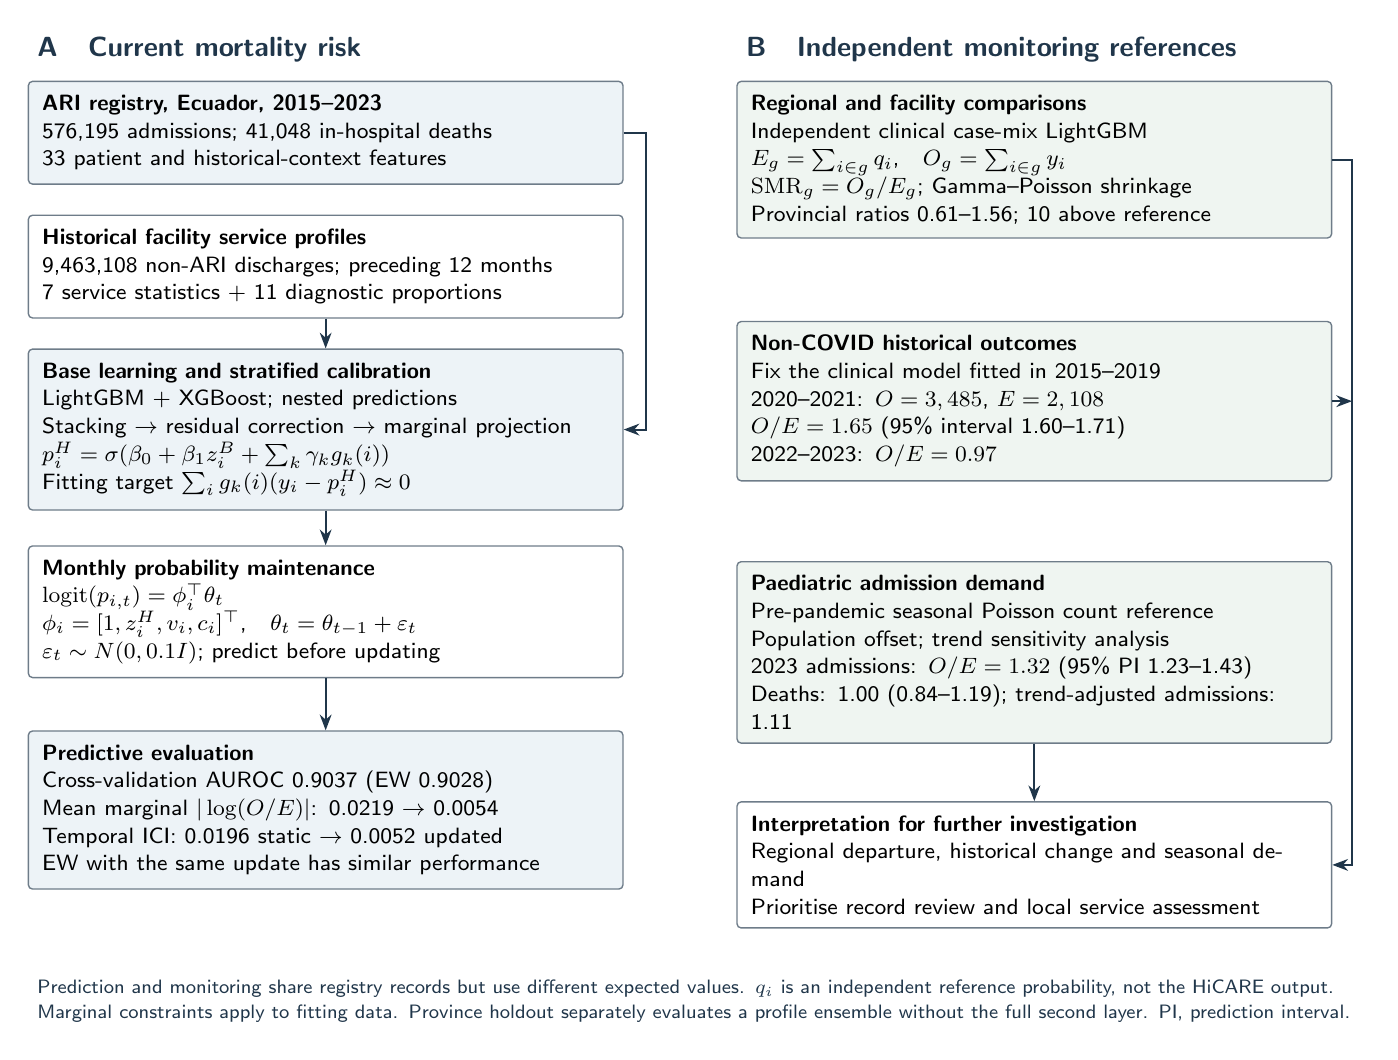
\begin{tikzpicture}[x=1cm,y=1cm]

\node[head] at (0,0) {A\quad Current mortality risk};
\node[head] at (9,0) {B\quad Independent monitoring references};
\node[box,text width=7.2cm,anchor=north west,fill=bluewash] (data) at (0,-.4) {\textbf{ARI registry, Ecuador, 2015--2023}\\576,195 admissions; 41,048 in-hospital deaths\\33 patient and historical-context features};
\node[box,text width=7.2cm,anchor=north west] (profile) at (0,-2.1) {\textbf{Historical facility service profiles}\\9,463,108 non-ARI discharges; preceding 12 months\\7 service statistics + 11 diagnostic proportions};
\node[box,text width=7.2cm,anchor=north west,fill=bluewash] (learn) at (0,-3.8) {\textbf{Base learning and stratified calibration}\\LightGBM + XGBoost; nested predictions\\Stacking $\to$ residual correction $\to$ marginal projection\\$p_i^H=\sigma(\beta_0+\beta_1z_i^B+\sum_k\gamma_kg_k(i))$\\Fitting target $\sum_i g_k(i)(y_i-p_i^H)\approx0$};
\node[box,text width=7.2cm,anchor=north west] (time) at (0,-6.3) {\textbf{Monthly probability maintenance}\\$\operatorname{logit}(p_{i,t})=\phi_i^\top\theta_t$\\$\phi_i=[1,z_i^H,v_i,c_i]^\top$,\quad $\theta_t=\theta_{t-1}+\varepsilon_t$\\$\varepsilon_t\sim N(0,0.1I)$; predict before updating};
\node[box,text width=7.2cm,anchor=north west,fill=bluewash] (eval) at (0,-8.65) {\textbf{Predictive evaluation}\\Cross-validation AUROC 0.9037 (EW 0.9028)\\Mean marginal $|\log(O/E)|$: 0.0219 $\to$ 0.0054\\Temporal ICI: 0.0196 static $\to$ 0.0052 updated\\EW with the same update has similar performance};
\node[box,text width=7.2cm,anchor=north west,fill=greenwash] (regional) at (9,-.4) {\textbf{Regional and facility comparisons}\\Independent clinical case-mix LightGBM\\$E_g=\sum_{i\in g}q_i$,\quad $O_g=\sum_{i\in g}y_i$\\$\mathrm{SMR}_g=O_g/E_g$; Gamma--Poisson shrinkage\\Provincial ratios 0.61--1.56; 10 above reference};
\node[box,text width=7.2cm,anchor=north west,fill=greenwash] (historic) at (9,-3.45) {\textbf{Non-COVID historical outcomes}\\Fix the clinical model fitted in 2015--2019\\2020--2021: $O=3,485$, $E=2,108$\\$O/E=1.65$ (95\% interval 1.60--1.71)\\2022--2023: $O/E=0.97$};
\node[box,text width=7.2cm,anchor=north west,fill=greenwash] (season) at (9,-6.5) {\textbf{Paediatric admission demand}\\Pre-pandemic seasonal Poisson count reference\\Population offset; trend sensitivity analysis\\2023 admissions: $O/E=1.32$ (95\% PI 1.23--1.43)\\Deaths: 1.00 (0.84--1.19); trend-adjusted admissions: 1.11};
\node[box,text width=7.2cm,anchor=north west] (use) at (9,-9.55) {\textbf{Interpretation for further investigation}\\Regional departure, historical change and seasonal demand\\Prioritise record review and local service assessment};
\draw[arr] (data.east)--++(.28,0)|-(learn.east); \draw[arr] (profile)--(learn); \draw[arr] (learn)--(time); \draw[arr] (time)--(eval);
\draw[arr] (regional.east)--++(.25,0)|-(use.east);
\draw[arr] (historic.east)--++(.25,0);
\draw[arr] (season)--(use);
\node[note,text width=16.8cm,anchor=north west] at (0,-11.7) {Prediction and monitoring share registry records but use different expected values. $q_i$ is an independent reference probability, not the HiCARE output. Marginal constraints apply to fitting data. Province holdout separately evaluates a profile ensemble without the full second layer. PI, prediction interval.};
\end{tikzpicture}\end{document}